%! Author = Omar Iskandarani
%! Title = Long-Distance Swirl Gravity from Chiral Swirling Knots with Central Holes
%! Date = Sept 25, 2025
%! Affiliation = Independent Researcher, Groningen, The Netherlands
%! License = © 2025 Omar Iskandarani. All rights reserved. This manuscript is made available for academic reading and citation only. No republication, redistribution, or derivative works are permitted without explicit written permission from the author. Contact: info@omariskandarani.com
%! ORCID = 0009-0006-1686-3961
%! DOI = 10.5281/zenodo.17328593

\newcommand{\paperversion}{\textbf{v0.0.2}} % Semantic versioning: vMAJOR.MINOR.PATCH
\newcommand{\papertitle}{Long-Distance Swirl Gravity from Chiral Swirling Knots with Central Holes}
\newcommand{\paperdoi}{10.5281/zenodo.17328593}

%========================================================================================
% PACKAGES AND DOCUMENT CONFIGURATION
%========================================================================================
\documentclass[11pt]{article}

% ====== minimal packages ======
\usepackage{amsmath,amssymb,amsfonts}
\usepackage{bm}
\usepackage{physics}
\usepackage{microtype}
\usepackage{tcolorbox}
\usepackage{hyperref}
\hypersetup{colorlinks=true,linkcolor=blue,citecolor=blue,urlcolor=blue}

% ==== Packages ====
\usepackage[T1]{fontenc}
\usepackage{lmodern}
\usepackage{booktabs}
\usepackage[utf8]{inputenc}
\usepackage[caption=false]{subfig}

% ===== Gauge sector macros =====
\renewcommand{\Tr}{\mathrm{Tr}}
\newcommand{\ii}{\mathrm{i}}
\newcommand{\GsA}{G^a_{\mu\nu}}
\newcommand{\WsI}{W^i_{\mu\nu}}
\newcommand{\Bmn}{B_{\mu\nu}}

% ===============================
% Macros (canonicalized)
% ===============================

% swirl arrows (context-aware)
\newcommand{\swirlarrow}{%
    \mathchoice{\mkern-2mu\scriptstyle\boldsymbol{\circlearrowleft}}%
    {\mkern-2mu\scriptstyle\boldsymbol{\circlearrowleft}}%
    {\mkern-2mu\scriptscriptstyle\boldsymbol{\circlearrowleft}}%
    {\mkern-2mu\scriptscriptstyle\boldsymbol{\circlearrowleft}}%
}
\newcommand{\swirlarrowcw}{%
    \mathchoice{\mkern-2mu\scriptstyle\boldsymbol{\circlearrowright}}%
    {\mkern-2mu\scriptstyle\boldsymbol{\circlearrowright}}%
    {\mkern-2mu\scriptscriptstyle\boldsymbol{\circlearrowright}}%
    {\mkern-2mu\scriptscriptstyle\boldsymbol{\circlearrowright}}%
}

% Canonical symbols
\newcommand{\vswirl}{\mathbf{v}_{\swirlarrow}}
\newcommand{\vswirlcw}{\mathbf{v}_{\swirlarrowcw}}
\newcommand{\SwirlClock}{S_{(t)}^{\swirlarrow}}
\newcommand{\SwirlClockcw}{S_{(t)}^{\swirlarrowcw}}
\newcommand{\omegas}{\boldsymbol{\omega}_{\swirlarrow}}  % swirl vorticity
\newcommand{\vscore}{v_{\swirlarrow}}                    % shorthand: |v_swirl| at r=r_c
\newcommand{\vnorm}{\lVert \mathbf{v}_{\mkern-2mu\scriptscriptstyle\boldsymbol{\circlearrowleft}} \rVert}               % swirl speed magnitude
\newcommand{\rhof}{\rho_{\!f}}                           % effective fluid density
\newcommand{\rhoE}{\rho_{\!E}}                           % swirl energy density
\newcommand{\rhom}{\rho_{\!m}}                           % mass-equivalent density
\newcommand{\rhocore}{\rho_{\mathrm{core}}}
\newcommand{\rc}{r_c}                                    % string core radius (swirl string radius)
\newcommand{\FmaxEM}{F_{\mathrm{EM}}^{\max}}             % EM-like maximal force scale
\newcommand{\FmaxG}{F_{\mathrm{G}}^{\max}}               % G-like maximal force scale
\newcommand{\Lam}{\Lambda}                               % Swirl Coulomb constant
\newcommand{\Om}{\Omega_{\swirlarrow}}                   % swirl angular frequency profile
\newcommand{\alpg}{\alpha_g}                             % gravitational fine-structure analogue
% --- Minimal macro prelude (safe, local) ---
\providecommand{\rc}{r_c}
\newcommand{\omegaVec}{\boldsymbol{\omega}}
\newcommand{\rhoF}{\rho_{\!f}}     % effective fluid density
\newcommand{\rhoM}{\rho_{\!m}}     % mass-equivalent density
\newcommand{\OmegaCore}{\Omega_{\mathrm{core}}}
\newcommand{\bg}{\mathrm{bg}}
\newcommand{\core}{\mathrm{core}}
\newcommand{\GammaC}{\Gamma_C}

% ===============================
% Policy: the golden constant is only allowed via hyperbolic functions.
\newcommand{\xig}{\operatorname{asinh}\!\left(\tfrac{1}{2}\right)}
\newcommand{\phig}{\exp(\xig)}
\newcommand{\phialg}{\bigl(1+\sqrt{5}\bigr)/2}
\newcommand{\xigold}{\tfrac{3}{2}\,\xig}
\newcommand{\GoldenDeclare}{%
    \textbf{Golden (hyperbolic)}:\ \(\ln\phi=\xig\), hence \(\phi=\phig\).
    \ \emph{(Equivalently, \(\phi=\phialg\); the algebraic form is derivative.)}%
}
\usepackage{graphicx}
\usepackage{geometry}
\geometry{margin=1in}

\usepackage{tikz}
\usetikzlibrary{calc,arrows.meta,decorations.markings,decorations.pathmorphing,
                decorations.pathreplacing,intersections,knots,hobby,shapes.geometric}
% If you actually need spath3, load it as a package (comment out if not installed):
% \usepackage{spath3}


% A tiny style for loop arrows
\tikzset{
    looparrow/.style={-{Stealth[length=2.5mm,width=1.8mm]},thick},
    knotline/.style={ultra thick, blue!70},
    testloopON/.style={thick, draw=green!60!black},
    testloopOFF/.style={thick, draw=red!70},
    axes/.style={very thick, black},
}

\usepackage{siunitx}
\AtBeginDocument{\RenewCommandCopy\qty\SI}

% Styling helpers
\tikzset{
    axisline/.style={very thick, black},
    corecircle/.style={thick, dashed, gray},
    knotline/.style={ultra thick, blue!65},
    swirlarrow/.style={-{Stealth[length=3mm,width=2mm]}, thick},
    vline/.style={-{Stealth[length=3mm,width=2mm]}, thick, teal!70!black},
    tube/.style={line width=6pt, line cap=round},
    ghost/.style={opacity=0.25},
    labelbox/.style={fill=white, inner sep=2pt, rounded corners=2pt},
}


% ------- Shared styles  -------
\tikzset{
    knot diagram/every strand/.append style={
        line cap=round,
        line join=round,
        ultra thick,
        red
    },
    every knot/.style={line cap=round,line join=round,very thick},
    strand/.style={line cap=round,line join=round,line width=3pt,draw=black},
    over/.style={preaction={draw=white,line width=6.5pt}},
}
\newcommand{\titlepageOpen}{
  \begin{titlepage}
  \thispagestyle{empty}
  \centering
  {\Large\bfseries Long-Distance Swirl Gravity from Chiral Swirling Knots with Central Holes \par}
  \vspace{1cm}
  {\Large\itshape \textbf{Omar Iskandarani}\textsuperscript{\textbf{*}} \par}
  \vspace{0.5cm}
  {\today \par}
  \vspace{0.5cm}
}

% here comes abstract
\newcommand{\titlepageClose}{
     \vfill
      \raggedright % <-- fixes left alignment
      \null
      \begin{picture}(0,0)
      % Adjust position: (x,y) = (left, bottom)
      \put(0,-45){  % Shift 200pt left, 40pt down
        \begin{minipage}[b]{0.7\textwidth}
        \footnotesize % One step bigger than \tiny \scriptsize
        \renewcommand{\arraystretch}{1.0}
        \noindent\rule{\textwidth}{0.4pt} \\[0.5em]  % ← horizontal line
        \textsuperscript{\textbf{*}} Independent Researcher, Groningen, The Netherlands \\
        Email: \texttt{info@omariskandarani.com} \\
        ORCID: \texttt{\href{https://orcid.org/0009-0006-1686-3961}{0009-0006-1686-3961}} \\
        DOI: \href{https://doi.org/\paperdoi}{\paperdoi} \\
        \textbf{Keywords:} Swirl-String Theory, Topological Gravity, Entropic Force, Circulation Quantization, Flat-Space Field Theory
        \end{minipage}
      }
      \end{picture}
      \end{titlepage}
}

\begin{document}
\titlepageOpen

    \begin{abstract}
    In Swirl–String Theory (SST), long-range attraction arises from the topology of \emph{chiral swirling knots}—vortex filaments including the trefoil (\(3_1\)), cinquefoil (\(5_1\)), \(5_2\), and stevedore (\(6_1\)). Each knot surrounds a straight rotation axis that carries the circulation. By Cauchy’s integral theorem~\cite{ahlforsComplexAnalysis1979,cauchy1825}, loops that link this axis exhibit an integer plateau of circulation, which we record with the Swirl Clock \(\SwirlClock\). When two composite tubes (e.g., the proton cores in H\(_2\)) share a central axis across an equal-pressure boundary, additive circulation deepens the common pressure well, consistent with attraction between neutral molecules in flat space~\cite{london1930,casimirpolder1948}. A crisp laboratory discriminator follows from the swirl–EM correspondence: topology changes in the swirl network generate geometry-independent, discrete electromotive impulses of fixed magnitude, \(\Delta\Phi=\pm\Phi_\star\)~\cite{DeaverFairbank1961,LittleParks1962}, with sign set by chirality. Non-integral steps, geometry-dependent amplitudes, or persistence without verified linking would falsify this mechanism.
    \end{abstract}


\section{Chiral Swirling Knots and Central Holes}
    Consider a chiral knot $K$ embedded in $\mathbb{R}^3$, such as Fig.~\ref{fig:knot-gallery}:

    \begin{figure}[htbp]
        \centering
        \subfloat[$3_1$ (trefoil)\label{fig:3-1}]{
            \includegraphics[width=0.22\linewidth]{figures/3_1}}
        \hfill
        \subfloat[$5_1$ (cinquefoil)\label{fig:5-1}]{
            \includegraphics[width=0.22\linewidth]{figures/5_1}}
        \hfill
        \subfloat[$5_2$ (cinquefoil twist)\label{fig:5-2}]{
            \includegraphics[width=0.22\linewidth]{figures/5_2}}
        \hfill
        \subfloat[$6_1$ (stevedore)\label{fig:6-1}]{
            \includegraphics[width=0.22\linewidth]{figures/6_1}}
        \caption{Canonical knot gallery.}
        \label{fig:knot-gallery}
    \end{figure}

    Each knot can be parametrized on a torus with major radius $R$ and minor radius $r$.
    The core tube of radius $r_c$ supports a tangential swirl velocity $\vswirl$, defining the \emph{Swirl Clock} $\SwirlClock$.

    A key structural feature is a \emph{central hole} threaded by a straight axis (taken as the $z$-axis), along which the analytic swirl potential is singular.
\titlepageClose

    \begin{figure}[t]
        \centering
        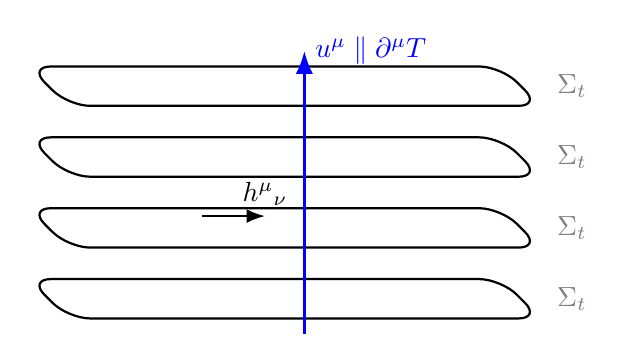
\begin{tikzpicture}[scale=1.0,>=Latex]
            \foreach \y in {0,0.9,1.8,2.7}{
                \draw[rounded corners=8pt,thick] (-3,\y) -- (3,\y) -- (2.5,\y+0.5) -- (-3.5,\y+0.5) -- cycle;
                \node[gray] at (3.4,\y+0.25) {$\Sigma_{t}$};
            }
            \draw[->,very thick,blue] (0,-0.2) -- (0,3.4) node[right] {$u^\mu \parallel \partial^\mu T$};
            \draw[->,thick] (-1.3,1.3) -- (-0.5,1.3) node[above] {$h^\mu{}_\nu$};
        \end{tikzpicture}
        \caption{Preferred foliation by the clock field $T(x)$ with unit timelike $u^\mu$, and spatial projector $h_{\mu\nu}=g_{\mu\nu}+u_\mu u_\nu$.}\label{fig:foliation}
    \end{figure}

    % ============================
    % Figure: Trefoil + central axis + circulation loops (clean, layered)
    % ============================

    \begin{figure}[htbp]
      \centering
      \includegraphics[width=0.7\linewidth]{figures/trefoil_axis_plateu}
            \caption{Trefoil knot with central axis and circulation loops in the \(z{=}0\) plane.
            Loops whose spanning disk intersects the filament within the torus annulus measure a plateau \(\Gamma=\mathrm{Lk}\cdot\kappa=\pm 3\,\kappa\) (sign by orientation).
            Loops outside the annulus do not enclose the filament and give \(\Gamma\approx 0\).}
            \label{fig:trefoil_axis_plateau_clean}
    \end{figure}


\section{Cauchy Integral and Circulation Quantization}
    Let $C$ be a closed loop in the $x$–$y$ plane encircling the $z$-axis. For an analytic swirl potential $W(z)=\Phi+i\Psi$ in a simply connected region,
    \begin{equation}
        \oint_C \vswirl \cdot d\mathbf{l} =
        \begin{cases}
            0, & \text{if no singularity inside,}\\[4pt]
            2\pi i\, \mathrm{Res}\!\left(\frac{dW}{dz}, z=0\right), & \text{if the axis is enclosed.}
        \end{cases}\label{eq:cauchy-circulation}
    \end{equation}
    In SST we identify the residue with a circulation quantum $\kappa$. Independently of the complex-potential language, Kelvin’s theorem fixes circulation~\cite{helmholtz1858,kelvin1869,Saffman1992,MajdaBertozzi2002} on any material loop; both viewpoints agree on the integer plateau:
    \begin{equation}
        \Gamma_C = n\,\kappa \quad \text{if the loop links $n$ times with the core.}
        \label{eq:circulation-quantization}
    \end{equation}

    \begin{tcolorbox}[title=\textbf{Canonical identification of $\kappa$ (SST)}]
        We adopt the equivalence
        \[
            \boxed{\;\kappa \equiv \frac{h}{m_{\text{eff}}} \;=\; 2\pi\, r_c\, v_c\;}
        \]
        which gives a direct bridge between the quantum of circulation and core kinematics. Hence
        \[
            m_{\text{eff}} \;=\; \frac{h}{2\pi r_c v_c}\,.
        \]
        \textbf{Numerics (SI):} with $r_c=\qty{1.40897017e-15}{m}$ and $v_c=\lVert \mathbf{v}_{\swirlarrow}\rVert=\qty{1.09384563e6}{m/s}$,
        \[
            \kappa=2\pi r_c v_c=\qty{9.6836192e-9}{m^2/s},\qquad
            m_{\text{eff}}=\frac{h}{\kappa}=\qty{6.842555e-26}{kg}\approx\qty{38.384}{GeV/c^2}.
        \]
    \end{tcolorbox}

    \noindent\emph{Status/limits:} Dimensions are consistent ($[\kappa]=L^2T^{-1}$). For loops whose spanning disk intersects the torus annulus of the filament, $\Gamma$ plateaus at $n\kappa$; for loops entirely outside, $\Gamma\approx 0$ (as illustrated in Fig.~\ref{fig:trefoil_axis_plateau_clean}).

    \begin{tcolorbox}[title=\textbf{Swirl–EM correspondence (operational note)}]
        In the Canon’s swirl–EM mapping, time-varying core areal density acts as a “source” via a term of the form $b^{\swirlarrow}=G^{\swirlarrow}\,\partial_t \varrho^{\swirlarrow}$, providing a handle for experimental couplings. Dynamics on the central line that modulate $\varrho^{\swirlarrow}$ can therefore seed measurable EM-like responses without curving space, consistent with the flat-space treatment used here.
    \end{tcolorbox}

\section{Composite Baryon Tubes}
    Inside baryons, three quark knots (e.g., $5_2$, $5_2$, $6_1$; see Figs.~\ref{fig:5-2} and \ref{fig:6-1}) meet at a Y-shaped junction, forming a single composite swirl tube (Fig.~\ref{fig:three-knot-gallery}).

    \begin{figure}[htbp]
        \centering
        \subfloat[Top view of 3 quark knots\label{fig:baryon}]{
            \includegraphics[width=0.3\linewidth]{figures/sst_three_knot_180_speed_stagnation}}
        \subfloat[3D view of 3 quark knots\label{fig:baryon3d1}]{
            \includegraphics[width=0.3\linewidth]{figures/sst_three_knot_3d_streamlines_colored_ULTRALIGHT}}
        \subfloat[Composite tube\label{fig:baryon_composite_tube}]{

            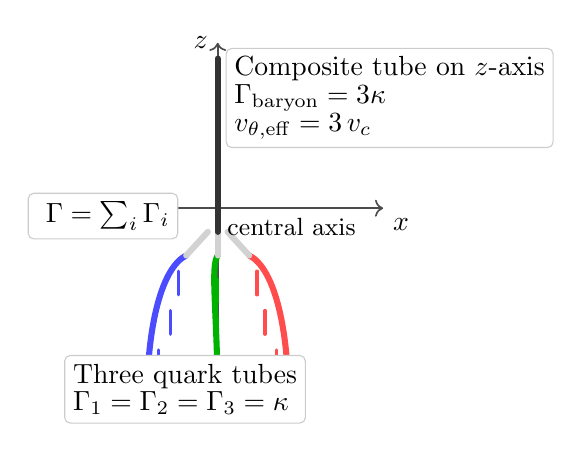
\begin{tikzpicture}[scale=0.5, line cap=round, line join=round]

                \tikzset{
                    axisline/.style={draw=black!70, line width=0.6pt},
                    tube/.style={draw, line width=2.2pt, rounded corners=2pt},
                    vline/.style={draw, line width=1.2pt},
                    labelbox/.style={fill=white, draw=black!20, rounded corners=2pt, inner sep=3pt}
                }

                \draw[axisline, ->] (0,-5.2) -- (0,4.2) node[left] {$z$};
                \draw[axisline, ->] (-4.2,0) -- (4.2,0) node[below right] {$x$};
                \fill (0,0) circle (2pt);


                % ---------- Three incoming quark tubes (from -z, merging to z-axis) ----------
                \draw[tube, blue!70]
                (-1.8,-5.0) .. controls + (0,2.1) and +(-0.6,-0.3) .. (-0.8,-1.2);
                \draw[tube, green!70!black]
                (0.0,-5.0) .. controls + (0,2.3) and +(-0.2,-0.3) .. (0.0,-1.2);
                \draw[tube, red!70]
                (1.8,-5.0) .. controls + (0,2.1) and +(0.6,-0.3) .. (0.8,-1.2);

                % ---------- Y-junction region into the central tube ----------
                \draw[tube, gray!35] (-0.8,-1.2) -- (-0.25,-0.6);
                \draw[tube, gray!35] ( 0.0,-1.2) -- ( 0.0,-0.6);
                \draw[tube, gray!35] ( 0.8,-1.2) -- ( 0.25,-0.6);

                % ---------- Composite tube along +z on the central axis ----------
                \draw[tube, black!80]
                (0.0,-0.6) .. controls +(0,0.9) and +(0,-0.9) .. (0.0,3.8);

                % ---------- Swirl/flow direction tick marks ----------
                % Incoming (upwards along +z)
                \foreach \x/\z in {-1.5/-4.2, -1.2/-3.2, -1.0/-2.2}{
                    \draw[vline, blue!70] (\x,\z) -- ++(0,0.6);
                }
                \foreach \x/\z in {0.0/-4.4, 0.0/-3.4, 0.0/-2.4}{
                    \draw[vline, green!70!black] (\x,\z) -- ++(0,0.6);
                }
                \foreach \x/\z in {1.5/-4.2, 1.2/-3.2, 1.0/-2.2}{
                    \draw[vline, red!70] (\x,\z) -- ++(0,0.6);
                }
                % Composite (upwards along +z)
                \foreach \z in {-0.2, 0.8, 1.8, 2.8}{
                    \draw[vline, black!80] (0.0,\z) -- ++(0,0.8);
                }

                % ---------- Labels ----------
                \node[below right] at (0,0) {\small central axis};
                \node[align=left, labelbox, anchor=west] at (-3.9,-4.6) {Three quark tubes\\[-2pt]
                    \(\Gamma_1=\Gamma_2=\Gamma_3=\kappa\)};
                \node[align=left, labelbox, anchor=west] at (0.2,2.8) {Composite tube on \(z\)-axis\\[-2pt]
                    \(\Gamma_{\text{baryon}}=3\kappa\)\\[-2pt]
                    \(v_{\theta,\mathrm{eff}}=3\,v_c\)};
                \node[align=left, labelbox, anchor=east] at (-1,-0.2) { \(\ \Gamma=\sum_i \Gamma_i\)};
            \end{tikzpicture}
        }
        \caption{Baryon core as a \emph{composite swirl tube}. Three quark tubes (bottom) join via a Y-junction into a single tube along $+z$. Circulation adds linearly, $\Gamma_\text{baryon}=3\kappa$, hence $v_\theta , \textrm{eff}=\Gamma_\text{baryon}/(2\pi r_\text{eff})$ with $r_\text{eff}\approx r_c$ to leading order.}
        \label{fig:three-knot-gallery}
    \end{figure}

    Each quark knot $i$ has circulation $\Gamma_i = \kappa$ around the central axis (Fig.~\ref{fig:baryon_composite_tube}).
    By Kelvin’s theorem (linearity of circulation),
        \begin{equation}
            \Gamma_{\mathrm{baryon}}=\Gamma_1+\Gamma_2+\Gamma_3=3\kappa.
        \end{equation}
        Since $\Gamma=2\pi r\,v_\theta$,
        \begin{equation}
            \boxed{\;
            v_{\theta,\mathrm{eff}}=\frac{\Gamma_{\mathrm{baryon}}}{2\pi\,r_{\mathrm{eff}}}
                =\frac{3\kappa}{2\pi\,r_{\mathrm{eff}}}\,,
                \;}\label{eq:baryon-vtheta}
        \end{equation}
        with $r_{\mathrm{eff}}$ the effective core radius of the merged tube. In the thin-core, near-Rankine limit $r_{\mathrm{eff}}\approx r_c$ to leading order (so that $v_{\theta,\mathrm{eff}}\approx 3 v_c$ holds as a first-order estimate), while the deeper pressure well is set by the increased $\Gamma$.

        \paragraph{Swirl Clock scaling.}
        The Swirl Clock relation becomes
        \begin{equation}
            dt_{\mathrm{local}} = dt_\infty \sqrt{1 - \frac{(3 v_c)^2}{c^2}},\label{eq:baryon-swirl-clock}
        \end{equation}
        predicting a more pronounced local time dilation, consistent with the larger rest mass of baryons relative to single quark knots.

            \emph{Analogy (for intuition).} Three equal water whirls feed one outlet: the hole may widen slightly, but the combined spin deepens the whirl and speeds the rim roughly threefold.





\section{Swirl Gravity and Molecular Attraction}
    Two composite tubes (e.g., two protons) that share the same central line produce a combined circulation
    \[
        \Gamma_{\mathrm{total}} = (3 \kappa)_{\mathrm{proton}} + (3 \kappa)_{\mathrm{proton}} = 6 \kappa,
    \]
    which deepens the shared pressure well and yields a stronger long-range attraction.
    This is consistent with the observation that neutral molecules (e.g., H$_2$) attract in Euclidean space~\cite{london1930,casimirpolder1948}: their baryon cores can be connected by the same central line, with the resulting swirl contribution following from additive circulation.

    \subsection{Electromotive Response to Swirl Gravity}
        Recent work in the SST Canon~\cite{Iskandarani2025EMG} indicates that time-dependent swirl density $\partial_t \vec{\rho}_{\circlearrowleft}$ acts as a source term in a modified Faraday law:
        \[
            \nabla \times \vec{E} = -\partial_t \vec{B} - \vec{b}_{\circlearrowleft}, \quad \vec{b}_{\circlearrowleft} = G_{\circlearrowleft} \, \partial_t \vec{\rho}_{\circlearrowleft}\label{eq:modified-faraday}
        \]
        Here, $G_{\circlearrowleft}$ is a universal topological transduction constant, canonically normalized to a flux quantum $\Phi^\star \in \{ h/e, h/2e \}$.
        For the formal derivation, see Appendix~\ref{sec:canonical-derivation-of-the-emswirl-coupling}.
        This coupling leads to a falsifiable prediction: nucleation or reconnection of vortex lines produces a quantized electromotive impulse of magnitude $\Phi^\star$. In gravitational contexts, pressure or density changes that alter swirl topology should have electromagnetic correlates. Thus, SST gravity is fluid-mechanical and electromagnetically active—features that can be tested in vortex-generating platforms.

    \subsection*{Companion Paper Reference}
        The modified Faraday law~\cite{Iskandarani2025EMG} with the swirl–induced source term~\eqref{eq:modified-faraday} is derived in a companion manuscript~\cite{Iskandarani2025EMG}. There, it is shown that $G_{\!\boldsymbol{\circlearrowleft}}$ is quantized in Weber units and identified with a flux quantum~\cite{DeaverFairbank1961,LittleParks1962}, $G_{\!\boldsymbol{\circlearrowleft}} = \Phi_\star \in \{h/e,\,h/2e\}$. In the present work we focus on experimental implications.


\section{Experimental Realization of Swirl-Induced Electromotive \mbox{Impulses}
}
\label{sec:exp-impulses}

    \subsection{Prediction}
    Topological transitions in the swirl sector (nucleation, annihilation, reconnection of swirl lines)
    generate quantized electromotive impulses,
    \begin{equation}
    \Delta\Phi = \pm\,\Phi_\star,
    \qquad
    \Phi_\star \in \Bigl\{ \tfrac{h}{e},\,\tfrac{h}{2e}\Bigr\},
    \end{equation}
    observable in any linked detection loop, independent of loop geometry. The sign of the impulse is set
    by chirality.

    \subsection{Condensed-Matter Implementation}
    Viable condensed-matter testbeds include:
    \begin{itemize}
        \item Type-II superconducting thin films with vortex entry/exit control,
        \item Quasi-2D atomic Bose–Einstein condensates,
        \item Magnetic skyrmion or Hopfion films.
    \end{itemize}
    A lithographed multi-turn superconducting micro-coil is positioned such that the defect line threads the
    loop during a topological transition. The induced impulse voltage is
    \begin{equation}
    V_{\text{imp}} \approx \frac{N \,\Phi_\star}{\Delta t},
    \end{equation}
    where $N$ is the number of turns and $\Delta t$ is the event timescale.

    \paragraph*{Numerical example.}
    For $N=1000$, $\Phi_\star = h/2e \approx 2.07\times10^{-15}\,\mathrm{Wb}$, and $\Delta t=10\,\mathrm{ns}$,
    \[
    V_{\mathrm{imp}} \approx 0.207\,\mathrm{mV}.
    \]
    For $\Delta t=1\,\mathrm{ns}$, $V_{\mathrm{imp}} \approx 2.07\,\mathrm{mV}$.

    \subsection{Protocol and Statistics}
    \begin{enumerate}
        \item Prepare the platform under controlled $(T,B,P)$.
        \item Trigger a single topological transition.
        \item Record the transient voltage.
        \item Repeat for $10^3$–$10^5$ events.
        \item Histogram the normalized flux $\int V(t)\,dt / N$.
    \end{enumerate}
    \textbf{Expected result:} discrete peaks at integer multiples of $\Phi_\star$, sign-flip under chirality
    reversal, invariance under linking-preserving deformations, collapse under unlinking or resistive replacement.

    \subsection{Hydrogenic and Atomic Systems}
    Swirl-Clock modulation predicts small line shifts in hydrogen, H$^-$, and H$_2$. High-resolution spectroscopy
    can be complemented with a micro-coil near the sample to detect coincident quantized impulses during
    internal topological transitions.

    \subsection{Falsifiability Criteria}
    \begin{itemize}
        \item Quantization: impulses in steps of $\Phi_\star$,
        \item Chirality: reversal flips sign,
        \item Linking number protection: preserved under deformations, destroyed by unlinking,
        \item Geometry independence: magnitude depends only on $N$ and $\Delta t$.
    \end{itemize}

\section{Galactic Rotation and Dark Matter Analogue}
\label{sec:galactic-dm}

    In addition to the molecular-scale picture, applying the same circulation quantization at galactic scales yields a two-component rotation profile that can reproduce flattened curves without introducing a separate non-baryonic halo \emph{within this model}.
    Let the azimuthal swirl velocity decompose into a core and a tail contribution:
    \begin{equation}
        v_\phi(r) \;=\; v_\text{core}(r) \;+\;
        C_\text{tail}\,\Big(1-e^{-r/\rc}\Big),
        \label{eq:core-tail}
    \end{equation}
    where $v_\text{core}(r)$ arises from finite baryonic-core circulation and the
    second term represents saturation of swirl transmission into the disk.

    \paragraph{Flat rotation curves.}
    In the limit $r\gg \rc$, Eq.~\eqref{eq:core-tail} asymptotes to
    \[
        v_\phi(r) \;\longrightarrow\; C_\text{tail},
    \]
    producing flattened rotation curves. This is a hydrodynamic consequence of circulation quantization and saturation in the present framework.

    \paragraph{Finite energy density.}
    The swirl energy density associated with the tail is
    \begin{equation}
        \rho_{\!E}(r) \;=\; \tfrac12\,\rhof\,v_\phi^2(r)
        \;\;\longrightarrow\;\; \tfrac12\,\rhof\,C_\text{tail}^2
        \quad (r\to\infty),
    \end{equation}
    which remains finite. Thus the apparent “dark halo” corresponds, in this model, to a constant swirl–energy plateau rather than an infinite mass distribution.

    \paragraph{Chirality selection.}
    Following the chiral–achiral selection principle developed in earlier VAM work, only \emph{chiral} knots couple coherently to the galactic swirl clock $S_t^{\boldsymbol{\circlearrowleft}}$. Achiral excitations (Fig.~\ref{fig:4-1}) fail to bind and are
    repelled from high–vorticity regions, precluding virialized halos.

    \begin{figure}[htbp]
      \centering
      \includegraphics[width=0.3\linewidth]{figures/4_1}
      \caption{An achiral \(4_1\) configuration (illustrative).}
      \label{fig:4-1}
    \end{figure}

    \paragraph{Rosetta consistency.}
    Using the Rosetta translation, the constants are fixed as
    \[
        \rhof \;=\; \frac{\rhocore\,\rc}{\lVert\mathbf{v}_{\!\boldsymbol{\circlearrowleft}}\rVert}\,\Omega,\qquad
        \rho_{\!E} \;=\; \tfrac12\,\rhof\,\lVert\mathbf{v}_{\!\boldsymbol{\circlearrowleft}}\rVert^2,\qquad
        \rho_{\!m} \;=\; \rho_{\!E}/c^2,
    \]
    ensuring dimensional consistency across both atomic (hydrogen) and galactic (rotational) scales.

    \paragraph{Falsifiers.}
    Two outcomes would challenge the proposal: (i) a system with well-measured baryons and negligible environmental coupling that still requires a full canonical dark-matter halo; (ii) a case where the inferred swirl coupling demands axis linkages that are topologically incompatible with the observed morphology.

    \paragraph{Summary.}
    Equation~\eqref{eq:core-tail} provides a falsifiable, SST-specific analogue of
    dark-matter phenomenology: flat galactic rotation curves, finite halo energy,
    and chirality-restricted matter coupling arise from quantized circulation in flat space.

\section{Entropic Embedding of Swirl–String Theory}
\label{sec:entropic-sst}
    Swirl–String Theory (SST), built on topologically quantized circulation in a flat, vortex-supporting medium, admits an entropic reinterpretation compatible with the core principles of emergent gravity \cite{verlinde2011origin,verlinde2016emergent,jacobson1995thermodynamics,padmanabhan2010thermodynamical,bekenstein1973black}, allowing mass, force, and time to be read as information-theoretic quantities.


    \subsection{Swirl Entropy as Informational Field}
        We define a swirl-based entropy field $S_{(x^\mu)}^{\swirlarrow} $ as a logarithmic function of the swirl areal density $\rho_{\swirlarrow} = \nabla \cdot \vec{a}$:

        \begin{equation}
            S_{(x^\mu)}^{\swirlarrow} = k_B \cdot \log\left(1 + \frac{\rho_{\swirlarrow}(x^\mu)}{\rho_0}\right)
        \end{equation}

        Here, $\rho_0$ is a baseline density. The field $S^{\swirlarrow} $ plays the role of a local entropy density, similar to that on a holographic screen in entropic gravity.

    \subsection{Entropic Force from Swirl Gradients}
        Verlinde’s entropic-force expression is:

        \begin{equation}
            F = T \cdot \frac{dS}{dx}
        \end{equation}

        In SST, circulation-induced pressure deficits are
        \begin{equation}
            \Delta p = -\frac{1}{2} \,\rhof\, v^2
        \end{equation}

        Assuming that swirl flow aligns with the entropy gradient, the effective force becomes
        \begin{equation}
            F_\text{swirl} \propto \nabla (\rhof v^2) \propto \nabla S^{\swirlarrow},
        \end{equation}
        establishing an explicit analogy between entropic forces and swirl-induced attraction in SST.

    \subsection{Mass as Topological Information}
        In SST, a mass scale is set by the circulation quantum $\kappa$:

        \begin{equation}
            m = \frac{h}{\kappa}, \qquad \kappa = 2\pi r_c v_c
        \end{equation}

        Interpreting $\kappa$ as a unit of quantized topological information, one may write a discrete sum over informational elements:

        \begin{equation}
            m_K = \sum_i \epsilon_i, \quad \epsilon_i = \frac{h}{\kappa_i}.
        \end{equation}

    \subsection{Time Dilation as an Entropic Clock}
        SST defines a Swirl Clock for local proper time,

        \begin{equation}
            dt_\text{local} = dt_\infty \sqrt{1 - \frac{v^2}{c^2}},
        \end{equation}

        consistent with entropic gravity, where time slows in regions of higher information density, i.e., larger $\rho_{\swirlarrow}$.

    \subsection{R/T Phase Transition and Information Localization}
        SST posits two phases:
        \begin{itemize}
        \item \textbf{R-phase}: unknotted, wave-like field state
        \item \textbf{T-phase}: knotted, particle-like topological excitation
        \end{itemize}

        The R-to-T transition represents entropic localization, akin to wavefunction collapse and decoherence, aligning SST with entropy-based emergence of space and matter.

    \subsection{Summary of Mapping}
        \begin{table}[h]
            \centering
            \begin{tabular}{lll}
                \toprule
                \textbf{SST Concept} & \textbf{Entropic Gravity Analog} & \textbf{Interpretation} \\
                \midrule
                $\rho_{\swirlarrow}$ & Entropy density & Local information field \\
                Swirl clock & Gravitational redshift & Entropic time rate \\
                $\Delta p$ & Entropic force & Gradient of entropy \\
                $\kappa$ & Info unit / bit & Mass from information \\
                R/T transition & Wave collapse & Information localization \\
                \bottomrule
            \end{tabular}
            \caption{Correspondences between SST and Verlinde's entropic gravity.}\label{tab:sst-entropic-mapping}
        \end{table}

        SST may therefore be read as an entropic field theory in flat space, where gravitational and inertial phenomena track topological and informational structures.

\section{Lagrangian and Action Formulation}
    The dynamical content of Swirl–String Theory (SST) can be expressed via an effective Lagrangian density $\mathcal{L}$ over flat spacetime, with swirl fields defined by a scalar potential $\phi(x^\mu)$, a swirl vector potential $a_\mu(x^\nu)$, and a fluid mass density field $\rhof$. Define the swirl areal density as $\rho_{\circlearrowleft} = \nabla \cdot \vec{a}$. With a Maxwell-like field strength
    \[
        F_{\mu\nu} = \partial_\mu a_\nu - \partial_\nu a_\mu,
    \]
    a representative Lagrangian is
    \[
        \mathcal{L}_{\text{SST}} = -\frac{1}{4} F_{\mu\nu} F^{\mu\nu} + \rhof\, (\partial_\mu \phi)(\partial^\mu \phi) - V(\phi) + \mathcal{L}_\text{topo},
    \]
    where $V(\phi)$ encodes a knot potential and $\mathcal{L}_\text{topo}$ collects topological couplings (e.g., braid index, genus).

    The action is then $S = \int \mathcal{L}_{\text{SST}} \, d^4x$. Euler–Lagrange equations yield conservation laws and dynamics for both swirl flow and its entropic analogs.

    In hydrogenic systems, swirl gradients around knot cores induce pressure deficits that couple to particle motion via Bernoulli–Euler dynamics, reproducing an effective gravitational behavior without spacetime curvature.

    \begin{quote}
    The quantized vortex mass formula, the swirl Schrödinger equation, and finite-core energy regularization were developed in the VAM framework~[Iskandarani, 2024]. The present work translates and updates these within SST notation via the Rosetta map~[Iskandarani, 2025]. % [EDIT] converted stray quotes to quote env; softened declarative tone
    \end{quote}



\section{Legacy Foundations and Rosetta Translation}
\label{sec:legacy-rosetta}

    The formal structure of Swirl–String Theory (SST) builds on a prior topological-fluid framework, the Vortex–Æther Model (VAM). That model derived physical results from circulation quantization and fluid field dynamics, including a topologically quantized mass formula, a swirl-based Schrödinger equation, and a non-divergent fluid Lagrangian. These are translated within SST via a symbolic mapping documented in the Rosetta file \cite{VAM-15, vamrosetta2025}.

    \subsection{Quantized Circulation and Mass Formula}

        In VAM, a core-mass mechanism arises from Onsager-like circulation quantization~\cite{onsager1949,feynman1955}:
        \begin{equation}
            \oint \vec{v} \cdot d\vec{\ell} = n \, \kappa_\text{\ae}
        \end{equation}
        with velocity expressed as a gradient,
        \begin{equation}
            \vec{v} = \lambda_\text{\ae} \, \nabla \theta, \qquad \psi = \sqrt{\rho/\rho_\text{\ae}}\, e^{i\theta},
        \end{equation}
        leading to a hydrodynamic Schrödinger equation with a swirl potential,
        \begin{equation}
            i\hbar_\text{\ae} \, \frac{\partial \psi}{\partial t} = -\frac{\hbar_\text{\ae}^2}{2m_\text{\ae}} \, \nabla^2 \psi + \Phi_{\text{swirl}}(\vec{\omega})\, \psi,
        \end{equation}
        \begin{equation}
            \Phi_{\text{swirl}} = \frac{1}{2} \, \lambda_g \, \rho_\text{\ae} \, |\vec{\omega}|^2.
        \end{equation}

        Reported vortex-mass estimates (e.g., for the electron) were within $\sim 10^{-7}$ of experimental values in that framework; independent verification is an open task.

    \subsection{Lagrangian and Field Formalism}

        VAM provided a fluid Lagrangian consistent with gauge-invariant dynamics:
        \begin{equation}
            \mathcal{L}_\text{VAM} = \frac{1}{2} \, \rhof \, (\nabla \times \vec{A})^2 + \rhof \, (\partial_t \phi)^2 - V(\phi).
        \end{equation}
        This maps to the SST flat-space field theory as
        \begin{equation}
            \mathcal{L}_\text{SST} = -\frac{1}{4} F_{\mu\nu} F^{\mu\nu} + \rhof \, (\partial_\mu \phi)(\partial^\mu \phi) - V(\phi) + \mathcal{L}_{\text{topo}},
        \end{equation}
        where the swirl vector $a_\mu$ replaces the VAM circulation potential, and $\mathcal{L}_{\text{topo}}$ incorporates topological invariants (braid index, genus, component count).

    \subsection{Notation Fidelity via Rosetta Map}

        All constants, fields, and structural equations have been translated via the VAM–SST Rosetta dictionary \cite{vamrosetta2025}, maintaining dimensional and symbolic consistency. This includes:
        \begin{itemize}
            \item Swirl velocity: $ \vec{v}_{\circlearrowleft} = \nabla \phi $
            \item Core swirl speed: $ \|\vec{v}_{\circlearrowleft}\| = 1.093 \times 10^6\ \text{m/s} $
            \item Core radius: $ r_c = 1.40897 \times 10^{-15}\ \text{m} $
            \item Core density: $ \rho_{\text{core}} = 3.89 \times 10^{18}\ \text{kg/m}^3 $
            \item Time variables: external time $ \tau$, swirl clock $ S(t)$, and proper loop time $ T_s $
        \end{itemize}

        This lineage yields a variational, quantized, and empirically calibrated foundation—recast here in a swirl-theoretic, flat-space field formalism.

\section{Conclusion}

    Long-distance attraction in SST is a manifestation of topological quantization: chiral knots with central holes enforce non-vanishing circulation residues along a central line.
    When multiple quark knots merge into a baryon, their circulations add linearly, forming a single composite tube with $3\kappa$ circulation.
    Two testable consequences follow: (1) discrete electromotive impulses of fixed magnitude $\Delta\Phi=\pm\Phi_\star$ at topology changes; (2) a contribution to large-scale dynamics that flattens rotation curves in systems with axis linkages.


\section*{Code and Data Availability}
    All predictive simulations used in this paper are implemented in the open Python script \texttt{SST\_INVARIANT\_MASS3.py}, available on request or at Zenodo: \url{https://doi.org/10.5281/zenodo.17155854}


\appendix

    \section{Canonical Derivation of the EM–Swirl Coupling (Summary from Canon)}
    \label{sec:canonical-derivation-of-the-emswirl-coupling}

        This appendix summarizes the canonical derivation of the EM–swirl coupling as developed in the
        \emph{Swirl–String Theory Canon}~\cite{Iskandarani_SST_Canon_v0_5_9_2025}. The goal is to show how
        time–dependent swirl density enters Maxwell–Faraday dynamics as an additional source term.

        \paragraph*{Swirl areal density.}
        A coarse–grained swirl density $\rho_{\circlearrowleft}(\mathbf{x},t)$ is defined as the number of
        quantized swirl lines per unit area. Its flux through a surface $S$ counts the number of vortex lines
        piercing $S$,
        \[
        \Phi_{\circlearrowleft}(t; S) = \int_S \rho_{\circlearrowleft} \, dA = N(S,t) \in \mathbb{Z}.
        \]
        Conservation of circulation (Kelvin invariant) ensures that $N$ is an integer topological quantity
        that can only change by nucleation, annihilation, or reconnection.\footnote{Full derivation available in the supplemental Canon document~\cite{Iskandarani_SST_Canon_v0_5_9_2025}.}

        \paragraph*{Modified Faraday law.}
        In a rotating–frame foliation, centrifugal and swirl–gravity effects unify into a single effective
        source $b_{\circlearrowleft}$. The Maxwell–Faraday curl equation becomes
        \[
        \nabla \times \mathbf{E} = -\partial_t \mathbf{B} - \mathbf{b}_{\circlearrowleft},
        \qquad
        \mathbf{b}_{\circlearrowleft} = G_{\circlearrowleft} \, \partial_t \rho_{\circlearrowleft}.
        \]
        Here $G_{\circlearrowleft}$ is a universal transduction constant with dimensions of Weber (V·s), so that
        $b_{\circlearrowleft}$ has the same units as $\partial_t B$ (V·m$^{-2}$).

        \paragraph*{Pillbox theorem.}
        Integrating over a surface $S$ and a time interval $[t_i,t_f]$ yields
        \[
        \int_{t_i}^{t_f} \!\! \oint_{\partial S} \mathbf{E}\cdot d\ell \, dt
        = - \Delta \Phi_B(S) - G_{\circlearrowleft}\, \Delta N(S),
        \]
        where $\Delta \Phi_B(S)$ is the magnetic flux change and $\Delta N(S)$ is the net change in vortex
        number through $S$. If the magnetic flux is held fixed, the time–integrated EMF reduces to a purely
        topological impulse proportional to $\Delta N$.

        \paragraph*{Normalization.}
        The Canon’s “electron logic’’ identifies one topological event ($\Delta N = \pm 1$) with a single flux
        quantum $\Phi_\star$. This fixes the constant to
        \[
        G_{\circlearrowleft} = \Phi_\star,
        \qquad
        \Phi_\star \in \Bigl\{ \tfrac{h}{e},\,\tfrac{h}{2e} \Bigr\},
        \]
        with the choice depending on whether the medium supports single–charge or Cooper–pair transport.
        This establishes that every topological transition injects a quantized EMF–time impulse, independent
        of drive details or geometry.

        \paragraph*{Dimensional consistency.}
        Since $[\rho_{\circlearrowleft}] = \text{m}^{-2}$ and $[\partial_t \rho_{\circlearrowleft}] =
        \text{m}^{-2}\text{s}^{-1}$, multiplying by $[G_{\circlearrowleft}] = \text{V·s}$ yields
        $[b_{\circlearrowleft}] = \text{V·m}^{-2}$, consistent with $[\partial_t B]$.

    \section{Rotating Frame and Flux Quantization}
    \label{sec:rotating-frame-and-flux-quantization}

        The rotating–frame derivation of the flux impulse is presented in full in the companion paper
        \cite{Iskandarani2025EMG}. The result is that each topological transition generates a quantized
        time–integrated electromotive force:
        \[
        \int V(t)\,dt = \Phi_\star \,\Delta N,
        \qquad
        \Phi_\star \in \left\{ \tfrac{h}{e}, \,\tfrac{h}{2e} \right\}.
        \]

        \paragraph*{Physical interpretation.}
        This law states that the EMF–time impulse is determined solely by the change in swirl line number
        ($\Delta N$) and the universal flux quantum $\Phi_\star$. The magnitude is independent of the loop
        geometry, linking details, or the microscopic rate of the event. Only the sign (set by chirality) and
        the integer $\Delta N$ matter.

        \paragraph*{Experimental implications.}
        In condensed–matter systems, controlled vortex entry or exit should yield measurable EMF impulses in
        linked pickup loops. The predicted size is $\sim$0.1–1 mV for $N=10^3$ turns and nanosecond-scale transitions,
        well within reach of SQUID or GHz digitizer detection.

        \paragraph*{Cosmological scaling.}
        At galactic scales, swirl nucleation or reconnection events during mergers should produce transient
        electromagnetic signatures. Their quantized character provides a falsifiable link between laboratory
        measurements and astrophysical phenomena.

        \paragraph*{Falsifiability.}
        Key experimental discriminants are: (i) quantization in units of $\Phi_\star$; (ii) chirality–dependent
        sign reversal; (iii) invariance under continuous loop deformations that preserve linking number; (iv)
        collapse of the signal if the loop is unlinked or resistive.

        These criteria connect the theoretical derivation of the swirl–EMF coupling directly to measurable
        laboratory and astrophysical observables.

        \paragraph*{Summary of Key Points.}
        \begin{itemize}
          \item Each topological swirl transition yields an impulse EMF \( \Delta \Phi = \pm \Phi_\star \).
          \item The signal is quantized, chirality-sensitive, and geometry-independent.
          \item Predictions apply across lab-scale and cosmic scales.
        \end{itemize}


\bibliographystyle{unsrt}
\bibliography{swirlgravity}



\end{document}